% 2007 年山东卷文科第 20 题：直四棱柱 ABCD-A1B1C1D1。
%   底面 ABCD 为直角梯形：AD⊥DC，AB∥DC，DC=DD1=2AD=2AB。
%   题（1）要证 D1C⊥AC1，（2）E 在 DC 上且 D1E∥平面 A1BD。
% 来源 PDF：gaokaomath-src/普通高考/2007/2007山东文.pdf
% SHA-256：64b760b73b0a8988bc87dd5d37fc646a10e257f357faf9ad7b1a17fdebaf4af3
% 原页：2007山东文.pdf 第 2 页（A3 三栏）第 1 栏，书页码 400。
% 重绘依据：斜投影，D(0,0)、C(2.2,0)，纵深向量 (0.55,0.75) 对应 AD=1，
%   AB=1 沿 DC 方向，DD1=2 竖直向上；被遮棱 DA、AB、AA1 画虚线，
%   题设辅助线 D1C、AC1、A1B、A1D、BD 均画出。
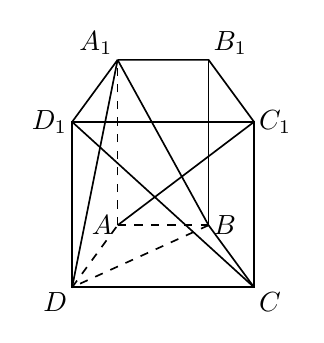
\begin{tikzpicture}[scale=1.05, semithick,
  every node/.style={inner sep=1.5pt}]
  \coordinate (D)  at (0,0);
  \coordinate (C)  at (2.2,0);
  \coordinate (A)  at (0.55,0.75);
  \coordinate (B)  at (1.65,0.75);
  \coordinate (D1) at (0,2.0);
  \coordinate (C1) at (2.2,2.0);
  \coordinate (A1) at (0.55,2.75);
  \coordinate (B1) at (1.65,2.75);

  % 被遮棱
  \draw[dashed] (D) -- (A);
  \draw[dashed] (A) -- (B);
  \draw[dashed] (A) -- (A1);
  % 题设辅助线
  \draw (D1) -- (C);
  \draw (A) -- (C1);
  \draw (A1) -- (B);
  \draw (A1) -- (D);
  \draw[dashed] (B) -- (D);
  % 可见棱
  \draw (D) -- (C) -- (C1) -- (D1) -- cycle;
  \draw (D) -- (D1);
  \draw (C) -- (C1);
  \draw (A1) -- (B1) -- (C1);
  \draw (A1) -- (D1);
  \draw (B1) -- (B);
  \draw (B) -- (C);

  % 顶点标注
  \node[below left]  at (D)  {$D$};
  \node[below right] at (C)  {$C$};
  \node[left]        at (A)  {$A$};
  \node[right]       at (B)  {$B$};
  \node[left]        at (D1) {$D_1$};
  \node[right]       at (C1) {$C_1$};
  \node[above left]  at (A1) {$A_1$};
  \node[above right] at (B1) {$B_1$};
\end{tikzpicture}
